\documentclass{article}
\usepackage{tikz}
\usepackage{graphicx}\usepackage{stix2}
\begin{document}
\pagenumbering{gobble}\[%\resizebox{30pc}{!}
\hspace{-10em}{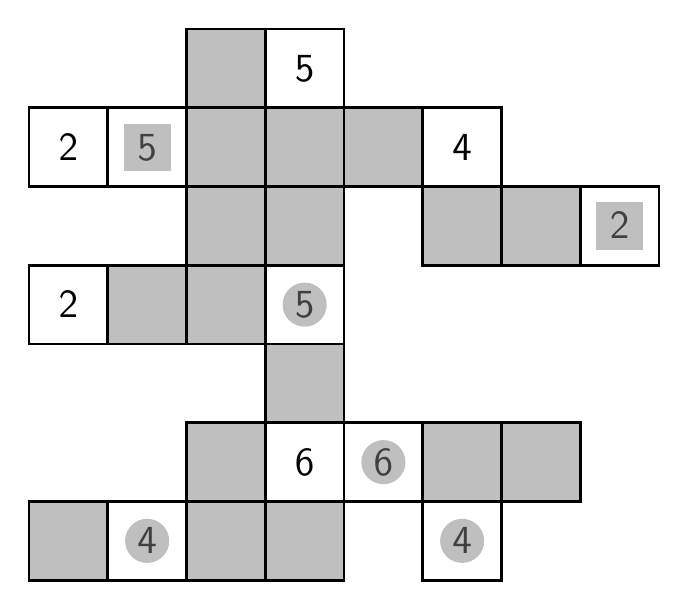
\begin{tikzpicture}\fill[gray, opacity = 0.5] (0, 0, 0)--++(1, 0, 0)--++(0, 1, 0)--++(-1, 0, 0)--cycle;
\draw[line width = 1pt] (0, 0, 0)--++(1, 0, 0)--++(0, 1, 0)--++(-1, 0, 0)--cycle;
\draw node at (1.5, 0.5, 0) {\Large $\mathsf{4}$};
\draw[line width = 1pt] (1, 0, 0)--++(1, 0, 0)--++(0, 1, 0)--++(-1, 0, 0)--cycle;
\fill[color = gray, opacity = 0.5] (1.5, 0.5, 0) circle (0.28);
\fill[gray, opacity = 0.5] (2, 0, 0)--++(1, 0, 0)--++(0, 1, 0)--++(-1, 0, 0)--cycle;
\draw[line width = 1pt] (2, 0, 0)--++(1, 0, 0)--++(0, 1, 0)--++(-1, 0, 0)--cycle;
\fill[gray, opacity = 0.5] (3, 0, 0)--++(1, 0, 0)--++(0, 1, 0)--++(-1, 0, 0)--cycle;
\draw[line width = 1pt] (3, 0, 0)--++(1, 0, 0)--++(0, 1, 0)--++(-1, 0, 0)--cycle;
\draw node at (5.5, 0.5, 0) {\Large $\mathsf{4}$};
\draw[line width = 1pt] (5, 0, 0)--++(1, 0, 0)--++(0, 1, 0)--++(-1, 0, 0)--cycle;
\fill[color = gray, opacity = 0.5] (5.5, 0.5, 0) circle (0.28);
\fill[gray, opacity = 0.5] (2, 1, 0)--++(1, 0, 0)--++(0, 1, 0)--++(-1, 0, 0)--cycle;
\draw[line width = 1pt] (2, 1, 0)--++(1, 0, 0)--++(0, 1, 0)--++(-1, 0, 0)--cycle;
\draw node at (3.5, 1.5, 0) {\Large $\mathsf{6}$};
\draw[line width = 1pt] (3, 1, 0)--++(1, 0, 0)--++(0, 1, 0)--++(-1, 0, 0)--cycle;
\draw node at (4.5, 1.5, 0) {\Large $\mathsf{6}$};
\draw[line width = 1pt] (4, 1, 0)--++(1, 0, 0)--++(0, 1, 0)--++(-1, 0, 0)--cycle;
\fill[color = gray, opacity = 0.5] (4.5, 1.5, 0) circle (0.28);
\fill[gray, opacity = 0.5] (5, 1, 0)--++(1, 0, 0)--++(0, 1, 0)--++(-1, 0, 0)--cycle;
\draw[line width = 1pt] (5, 1, 0)--++(1, 0, 0)--++(0, 1, 0)--++(-1, 0, 0)--cycle;
\fill[gray, opacity = 0.5] (6, 1, 0)--++(1, 0, 0)--++(0, 1, 0)--++(-1, 0, 0)--cycle;
\draw[line width = 1pt] (6, 1, 0)--++(1, 0, 0)--++(0, 1, 0)--++(-1, 0, 0)--cycle;
\fill[gray, opacity = 0.5] (3, 2, 0)--++(1, 0, 0)--++(0, 1, 0)--++(-1, 0, 0)--cycle;
\draw[line width = 1pt] (3, 2, 0)--++(1, 0, 0)--++(0, 1, 0)--++(-1, 0, 0)--cycle;
\draw node at (0.5, 3.5, 0) {\Large $\mathsf{2}$};
\draw[line width = 1pt] (0, 3, 0)--++(1, 0, 0)--++(0, 1, 0)--++(-1, 0, 0)--cycle;
\fill[gray, opacity = 0.5] (1, 3, 0)--++(1, 0, 0)--++(0, 1, 0)--++(-1, 0, 0)--cycle;
\draw[line width = 1pt] (1, 3, 0)--++(1, 0, 0)--++(0, 1, 0)--++(-1, 0, 0)--cycle;
\fill[gray, opacity = 0.5] (2, 3, 0)--++(1, 0, 0)--++(0, 1, 0)--++(-1, 0, 0)--cycle;
\draw[line width = 1pt] (2, 3, 0)--++(1, 0, 0)--++(0, 1, 0)--++(-1, 0, 0)--cycle;
\draw node at (3.5, 3.5, 0) {\Large $\mathsf{5}$};
\draw[line width = 1pt] (3, 3, 0)--++(1, 0, 0)--++(0, 1, 0)--++(-1, 0, 0)--cycle;
\fill[color = gray, opacity = 0.5] (3.5, 3.5, 0) circle (0.28);
\fill[gray, opacity = 0.5] (2, 4, 0)--++(1, 0, 0)--++(0, 1, 0)--++(-1, 0, 0)--cycle;
\draw[line width = 1pt] (2, 4, 0)--++(1, 0, 0)--++(0, 1, 0)--++(-1, 0, 0)--cycle;
\fill[gray, opacity = 0.5] (3, 4, 0)--++(1, 0, 0)--++(0, 1, 0)--++(-1, 0, 0)--cycle;
\draw[line width = 1pt] (3, 4, 0)--++(1, 0, 0)--++(0, 1, 0)--++(-1, 0, 0)--cycle;
\fill[gray, opacity = 0.5] (5, 4, 0)--++(1, 0, 0)--++(0, 1, 0)--++(-1, 0, 0)--cycle;
\draw[line width = 1pt] (5, 4, 0)--++(1, 0, 0)--++(0, 1, 0)--++(-1, 0, 0)--cycle;
\fill[gray, opacity = 0.5] (6, 4, 0)--++(1, 0, 0)--++(0, 1, 0)--++(-1, 0, 0)--cycle;
\draw[line width = 1pt] (6, 4, 0)--++(1, 0, 0)--++(0, 1, 0)--++(-1, 0, 0)--cycle;
\draw node at (7.5, 4.5, 0) {\Large $\mathsf{2}$};
\draw[line width = 1pt] (7, 4, 0)--++(1, 0, 0)--++(0, 1, 0)--++(-1, 0, 0)--cycle;
\fill[color = gray, opacity = 0.5] (7.2, 4.2) rectangle ++(0.6, 0.6);
\draw node at (0.5, 5.5, 0) {\Large $\mathsf{2}$};
\draw[line width = 1pt] (0, 5, 0)--++(1, 0, 0)--++(0, 1, 0)--++(-1, 0, 0)--cycle;
\draw node at (1.5, 5.5, 0) {\Large $\mathsf{5}$};
\draw[line width = 1pt] (1, 5, 0)--++(1, 0, 0)--++(0, 1, 0)--++(-1, 0, 0)--cycle;
\fill[color = gray, opacity = 0.5] (1.2, 5.2) rectangle ++(0.6, 0.6);
\fill[gray, opacity = 0.5] (2, 5, 0)--++(1, 0, 0)--++(0, 1, 0)--++(-1, 0, 0)--cycle;
\draw[line width = 1pt] (2, 5, 0)--++(1, 0, 0)--++(0, 1, 0)--++(-1, 0, 0)--cycle;
\fill[gray, opacity = 0.5] (3, 5, 0)--++(1, 0, 0)--++(0, 1, 0)--++(-1, 0, 0)--cycle;
\draw[line width = 1pt] (3, 5, 0)--++(1, 0, 0)--++(0, 1, 0)--++(-1, 0, 0)--cycle;
\fill[gray, opacity = 0.5] (4, 5, 0)--++(1, 0, 0)--++(0, 1, 0)--++(-1, 0, 0)--cycle;
\draw[line width = 1pt] (4, 5, 0)--++(1, 0, 0)--++(0, 1, 0)--++(-1, 0, 0)--cycle;
\draw node at (5.5, 5.5, 0) {\Large $\mathsf{4}$};
\draw[line width = 1pt] (5, 5, 0)--++(1, 0, 0)--++(0, 1, 0)--++(-1, 0, 0)--cycle;
\fill[gray, opacity = 0.5] (2, 6, 0)--++(1, 0, 0)--++(0, 1, 0)--++(-1, 0, 0)--cycle;
\draw[line width = 1pt] (2, 6, 0)--++(1, 0, 0)--++(0, 1, 0)--++(-1, 0, 0)--cycle;
\draw node at (3.5, 6.5, 0) {\Large $\mathsf{5}$};
\draw[line width = 1pt] (3, 6, 0)--++(1, 0, 0)--++(0, 1, 0)--++(-1, 0, 0)--cycle;
\end{tikzpicture}}\]

\vspace{5ex}

\[\resizebox{30pc}{!}{\begin{tikzpicture}\filldraw (1, 6, 0) circle (0.05);
\filldraw (0, 1, 0) circle (0.05);
\filldraw (6, 0, 0) circle (0.05);
\filldraw (2, 1, 0) circle (0.05);
\filldraw (3, 5, 0) circle (0.05);
\filldraw (0, 3, 0) circle (0.05);
\filldraw (3, 7, 0) circle (0.05);
\filldraw (4, 5, 0) circle (0.05);
\filldraw (4, 7, 0) circle (0.05);
\filldraw (5, 5, 0) circle (0.05);
\filldraw (1, 3, 0) circle (0.05);
\filldraw (6, 2, 0) circle (0.05);
\filldraw (2, 3, 0) circle (0.05);
\filldraw (6, 4, 0) circle (0.05);
\filldraw (1, 1, 0) circle (0.05);
\filldraw (7, 2, 0) circle (0.05);
\filldraw (3, 0, 0) circle (0.05);
\filldraw (7, 4, 0) circle (0.05);
\filldraw (0, 5, 0) circle (0.05);
\filldraw (4, 0, 0) circle (0.05);
\filldraw (1, 5, 0) circle (0.05);
\filldraw (4, 2, 0) circle (0.05);
\filldraw (5, 0, 0) circle (0.05);
\filldraw (2, 5, 0) circle (0.05);
\filldraw (6, 6, 0) circle (0.05);
\filldraw (5, 2, 0) circle (0.05);
\filldraw (4, 4, 0) circle (0.05);
\filldraw (2, 7, 0) circle (0.05);
\filldraw (8, 5, 0) circle (0.05);
\filldraw (3, 2, 0) circle (0.05);
\filldraw (4, 6, 0) circle (0.05);
\filldraw (3, 4, 0) circle (0.05);
\filldraw (0, 0, 0) circle (0.05);
\filldraw (3, 6, 0) circle (0.05);
\filldraw (0, 4, 0) circle (0.05);
\filldraw (1, 0, 0) circle (0.05);
\filldraw (7, 1, 0) circle (0.05);
\filldraw (5, 4, 0) circle (0.05);
\filldraw (0, 6, 0) circle (0.05);
\filldraw (5, 6, 0) circle (0.05);
\filldraw (2, 0, 0) circle (0.05);
\filldraw (6, 1, 0) circle (0.05);
\filldraw (2, 2, 0) circle (0.05);
\filldraw (6, 5, 0) circle (0.05);
\filldraw (2, 6, 0) circle (0.05);
\filldraw (3, 1, 0) circle (0.05);
\filldraw (1, 4, 0) circle (0.05);
\filldraw (7, 5, 0) circle (0.05);
\filldraw (3, 3, 0) circle (0.05);
\filldraw (4, 1, 0) circle (0.05);
\filldraw (2, 4, 0) circle (0.05);
\filldraw (4, 3, 0) circle (0.05);
\filldraw (5, 1, 0) circle (0.05);
\filldraw (8, 4, 0) circle (0.05);
\end{tikzpicture}}\]
\end{document}
